% reset section counter
\setcounter{section}{0}

%\metadata{lecture ID}{Your names}{date}
\metadata{9}{Rafael Rafailov and Aidan Perreault}{Feb 10th, 2021}

We now turn to a high-level overview of deep learning theory. To begin, we outline a framework for classical machine learning theory, then discuss how the situation is different from deep learning theory.

\sec{Framework for classical machine learning theory}
At the risk of oversimplification, we can divide classical machine learning theory into three parts:

\begin{enumerate}
\item {\bf Approximation theory} attempts to answer whether there is any choice of parameters $\theta$ that achieves low population error. In other words, is the choice of hypothesis class good enough to approximate the ground truth function? Using notation from earlier in this course, the goal is to upper bound $L(\theta^*) = \min_{\theta \in \Theta} L(\theta).$
    
\item {\bf Statistical generalization} focuses on bounding the excess risk $L(\hat{\theta}) - L(\theta^*)$. In Chapter \ref{chap:uc} we obtained the following bound:
    
\begin{equation}
L(\hat{\theta})-L(\theta^*)\leq \underbrace{L(\hat{\theta})-\hat{L}(\hat{\theta})}_{\text{generalization error}} + |L(\theta^*)-\hat{L}(\theta^*)|.
\end{equation}
    
The first term here is the generalization error, which usually has an upper bound of the form $R(\theta)/\sqrt{n}$, where $R(\theta)$ is some complexity measure.\footnote{In earlier chapters, we defined the complexity of a hypothesis class, not of a specific parameter value. To reconcile these two approaches, think of $R$ as a measure of complexity (such as a norm) that we can then use to define a hypothesis class $\Theta$, i.e.~$\Theta = \{\theta' : R(\theta') \le R(\theta)\}$.} This is a demonstration of \href{https://en.wikipedia.org/wiki/Occam%27s_razor}{\textit{Occam's Razor}}: the principle that simple (parsimonious, or low-complexity) explanations tend to generalize better. 
    
This statistical approach allows us to define a regularized loss  $\hat{L}_{\textup{reg}}(\theta)=\hat{L}(\theta)+\lambda R(\theta)$. Minimizing this loss gives us a solution $\hat{\theta}_\lambda$ which simultaneously has low training error and low complexity, which lets us bound both the training error and the generalization error. To summarize, in the classical setting, we can prove statements of the form
    
\begin{equation}\label{lec9:eqn:classical-guarantee}
\text{Any global minimizer }\hat{\theta}_\lambda \text{ of } \hat{L}_{\textup{reg}} \textup{ has small excess risk }  L(\hat{\theta}_\lambda) - L(\theta^*)\,.
\end{equation}

\item {\bf Optimization} considers how to obtain the minimizer $\hat\theta$ or $\hat{\theta}_\lambda$ computationally. This usually involves convex optimization: if $\hat{L}$ or $\hat{L}_{\textup{reg}}$ is convex, then we have a polynomial-time algorithm to find the global minimum.
\end{enumerate}

While there are many tradeoffs to consider between these three components (for example, we may be able to find a loss function for which optimization is easy, but generalization becomes worse), they are conceptually independent, and it is typically possible to study each area individually, then combine all three to get a result.

\sec{Deep learning theory and its differences}
The situation is more complex for deep learning theory. Two prominent differences are (a) the models are non-linear and the objective functions are non-convex, and (b) in deep learning, researchers have observed in many cases that more parameters typically help improve the performance, and many state-of-the-art models have much more parameters than the number of training data. (b) is often referred as to ``over-parameterization".

\begin{figure}[ht]
    \centerline{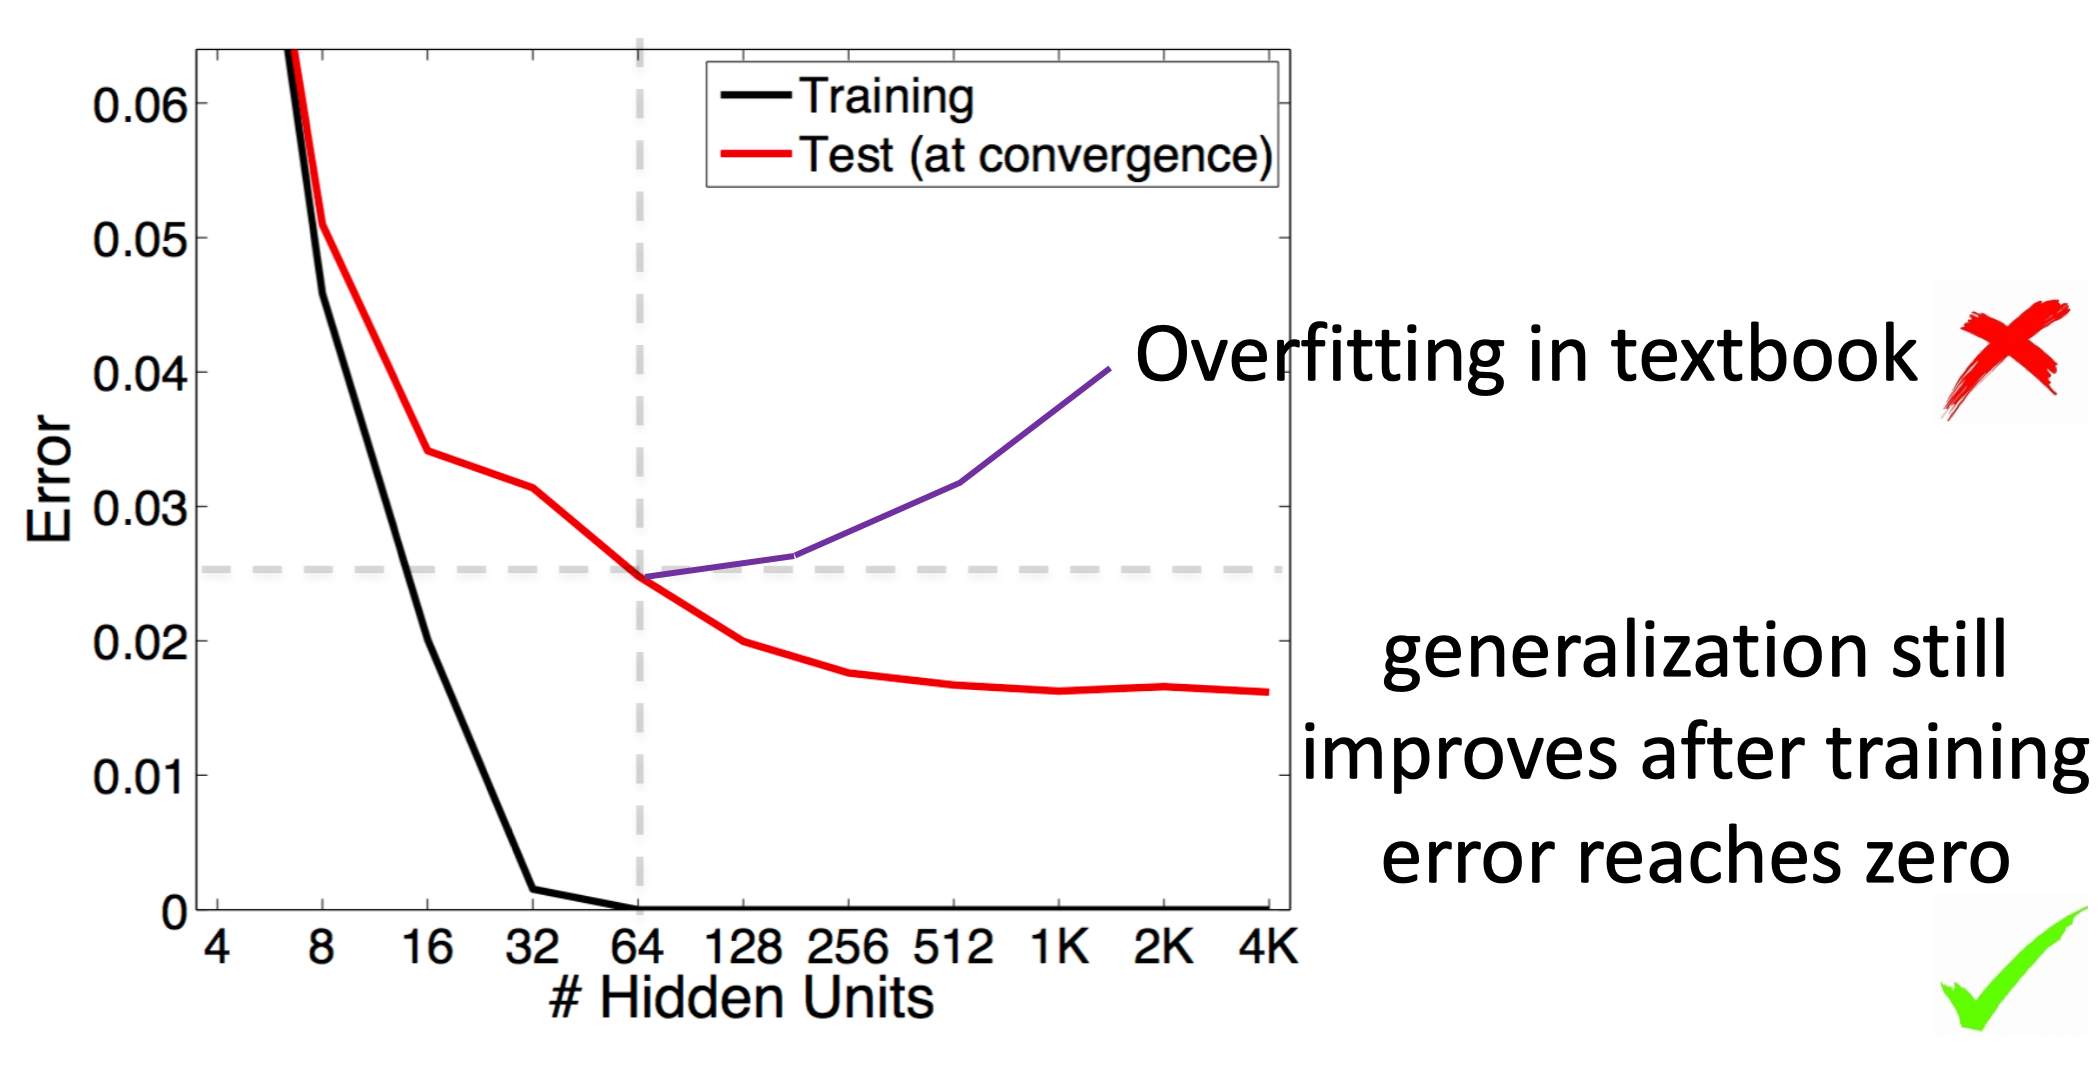
\includegraphics[width=4in]{figures/overparameterization.png}}
    \caption[lec9:fig:overparam]{The black and red lines denote the training and test error, respectively, of a three layer neural network fit to and evaluated on MNIST \cite{neyshabur2015norm}. While classical generalization theory predicts that beyond some threshold, the test error will increase with complexity (shown by the purple line), the true test error continues to decline with overparameterization. Though not depicted here, Neyshabur et al. observe similar test set error curves for a neural network fit to CIFAR-10.}
    \label{lec9:fig:overparam}
\end{figure}

Let us consider the difference in each of the three components described for classical machine learning theory. 

\begin{enumerate} 
\item {\bf Approximation theory:} Large neural net models are considered to be very expressive. That is, both the population loss $L(\theta)$ and the finite sample loss $\hat{L}(\theta)$ can be made small. In fact, neural networks are \textit{universal approximators}; see for example \cite{hornik1991}. This can be a somewhat misleading statement as the definition of universal approximator allows for the size of the network to be impracticably large, but morally it seems to hold true in practice anyway.
        
This expressivity is possible because neural networks are usually highly \textit{over-parametrized}: they have many more parameters than samples. It is possible to prove that in this regime, the network can ``memorize'' the entire dataset and achieve approximately zero training error \cite{arpit2017memorization}.
    
\item {\bf Statistical generalization:} Relatively weak regularization is used in practice. In many cases only weak $\ell_2$ regularization is used, i.e.
\begin{equation}
\widehat{L}_{\textup{reg}}(\theta)=\hat{L}(\theta)+\lambda\|\theta\|_2^2.
\end{equation}
    
The first interesting fact is that this regularized loss does not have a unique (approximate) global minimizer. This is due to overparametrization: there are so many degrees of freedom that there are many approximate global minimizers with approximately the same $\ell_2$ norm.
    
However, it turns out that these global minimizers are not equally good: many models which achieve zero training error may have very bad test error (Figure~\ref{lec9:fig:bad-global-min}). Take, for example, using stochastic gradient descent (SGD) to learn a model to classify the dataset CIFAR-10. In Figure~\ref{lec9:fig:dl-implicitreg}, we show two instantiations of this: one starting with a large learning rate and slowly decreasing it, and one with a small learning rate throughout. Even though both instantiations result in approximately zero training error, the former leads to much better test performance. 

Therefore, the job of optimizers in deep learning is not just to find an arbitrary global minimum: we need to find the right global minimum. This contrasts sharply with \eqref{lec9:eqn:classical-guarantee} from the classical setting, where achieving a global minimum leads to good guarantees on generalization error. This means that \eqref{lec9:eqn:classical-guarantee} is simply not powerful enough to deal with deep learning, because it cannot distinguish between global minima with good test error and bad test error.

\begin{figure}[t]
    \centering
    \begin{subfigure}[t]{0.49\textwidth}
        \centering
        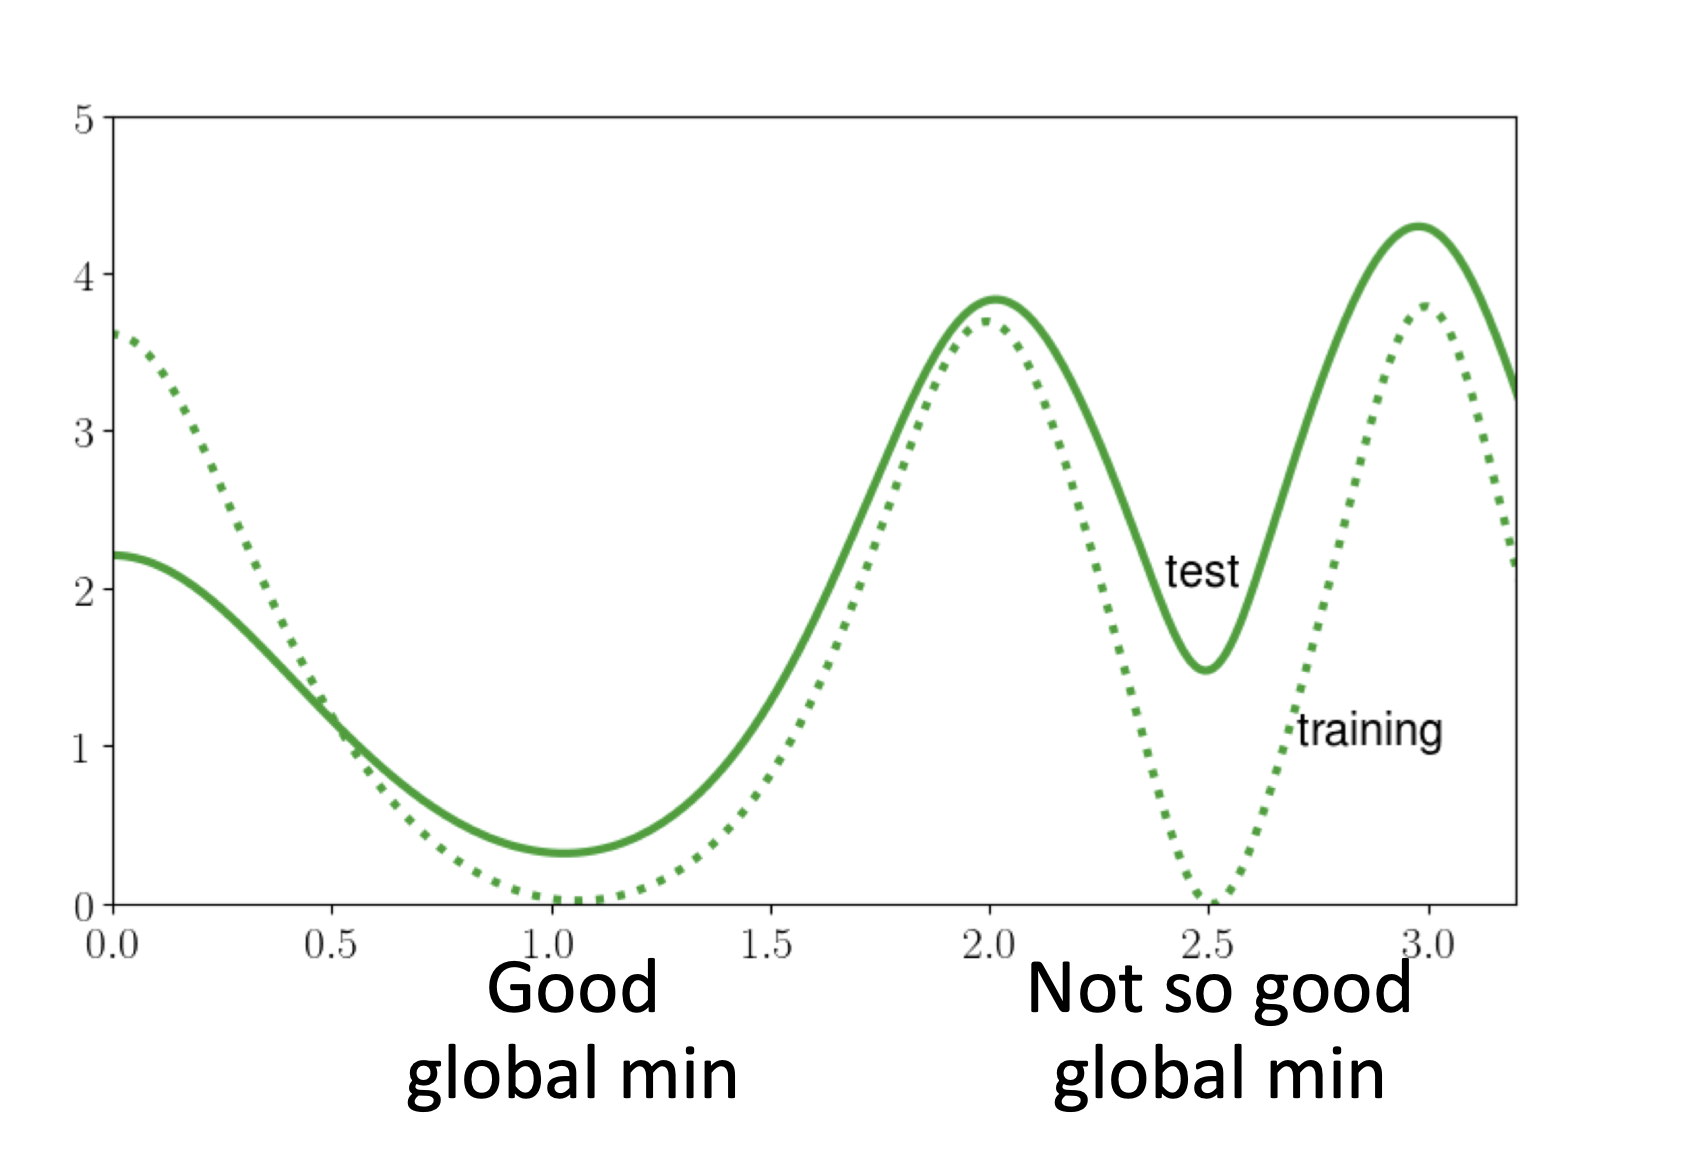
\includegraphics[width=3in]{figures/bad global min .png}
        \caption{}
        \label{lec9:fig:bad-global-min}
    \end{subfigure}
    \hfill
    \begin{subfigure}[t]{0.49\textwidth}
        \centering
        \hspace*{-1.8em}
        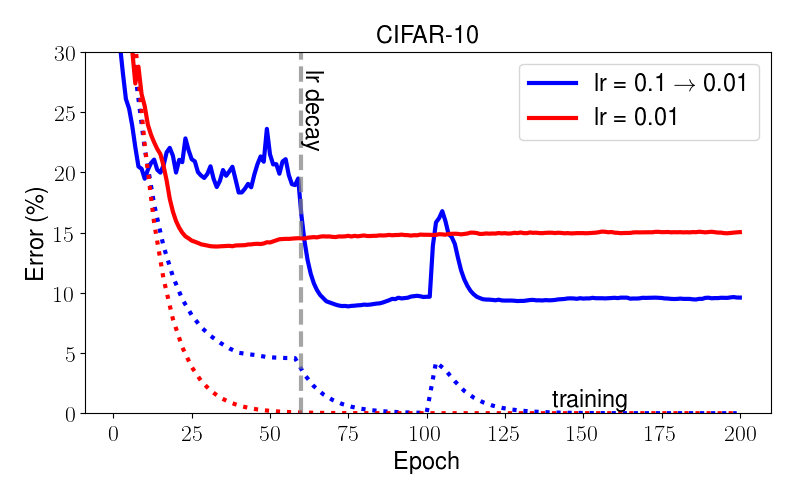
\includegraphics[width=3in]{figures/deep-learning-implicit-reg.png}
        \caption{}
        \label{lec9:fig:dl-implicitreg}
    \end{subfigure}
    \caption{We use dotted and solid lines to depict training and test error, respectively. Figure~\ref{lec9:fig:bad-global-min} demonstrates how global minimizers for the training loss can have differing performance on test data. In Figure~\ref{lec9:fig:dl-implicitreg}, blue and red colors differentiate between the model fit with a decaying learning rate and a small constant learning rate. Though both neural networks shown in this plot achieve 0 training error, the global minimizer obtained by a more sophisticated learning rate schedule appears to generalize better to unseen data.}
    \label{lec9:fig:global_min}
\end{figure}

\item {\bf Optimization:} The discussion above means that optimization plays a significant role in generalization for deep learning. Different training algorithms/optimizers have different ``implicit biases'' or ``implicit regularization effect'', causing them to converge to different global minimizers. Understanding the implicit regularization effect of optimizers is thus a central goal of deep learning theory. The lack of understanding implicit regularization hinders the development of fast optimizers---it is impossible to design a good optimization algorithm without also considering its impact on generalization. In fact, many algorithms for non-convex optimization have been proposed that work well for minimizing training loss, but because their implicit bias is different, they lead to worse test performance and are therefore not too useful.
    
Often these implicit biases or implicit regularization effect can be characterized in the form of showing the optimizers prefer $\hat\theta$ of certain low complexity among all the global minimizers. The deep learning analog of \eqref{lec9:eqn:classical-guarantee} often consists of two statements: (a) the optimizer implicitly prefers low complexity solution according to complexity measure $R(\cdot)$ by converging to a global minimizer $\hat{\theta}$ with low complexity $R(\hat{\theta})$, and (b) low complexity solutions generalize. This means that we end up doing more work on the optimization front---the optimizer needs to ensure both a small training loss and a low complexity solution. On the other hand, proving generalization bounds (statement (b)) works similarly to the classical setting once we understand how our optimizer finds a low-complexity solution.
    
\end{enumerate}

%To explain the success of deep learning, we will cover three tasks in the next two chapters\todo{specify chapter number}:
We summarize some of the results that we will present in the future chapters. \ttodo{add chapter number later}

\begin{enumerate}
    \item \textbf{Optimization.} First, we will prove that under certain data distribution assumption, optimizers such as stochastic gradient decent can converge to an approximate global minimum, even though the objective function is non-convex. Results of this form can be shown on matrix factorization problems and linearized neural networks, even without over-parameterization, but so far are limited to these simple models.  Second, we will discuss a recent approach, called neural tangent kernels (NTK), which proves that for almost any neural networks, with overparameterization, gradient descent can converge to a global minimum, \textit{under specific hyperparameter settings} (e.g, specific learning rate and initialization). However, it turns out that these specific hyperparaemeter settings \textit{does not} provide sufficient implicit regularization effect for the learned models to generalize. (In other words, the optimizer only returns a global minimizer, but not a global minimizer that generalizes well.)
    
    \item \textbf{Implicit regularization effect.} This involves showing that the solution $\hat{\theta}$ obtained by a particular optimizer has low complexity $R(\hat{\theta})\leq C$ according to some complexity measure $R(\cdot)$ (which depends on the choice of optimizers). It's believed and empirically observed that any changes or tricks in the optimizers (e.g., learning rate schedule, batch size, initialization, batchnorm) could introduce additional implicit regularization effects. We will only demonstrate these on some special cases of models (e.g. logistic regression, matrix factorization) and optimizers (e.g. gradient descent, label noise in SGD, dropout, learning rate). Recently, there are also more general results with label noise SGD~\citep{blanc2019implicit,damian2021label}. 
    
    \item \textbf{Generalization bounds.} This part involves showing that for all $\theta$ such that $R(\theta)\leq C$ with $\hat{L}(\theta)\approx 0$, we have $L(\theta)$ is small. That is, we show that low-complexity solutions to the empirical risk problem generalize well. We will be working with more fine-grained complexity measures (e.g., those complexity measures that are similar to the complexity measure in part 2 above that are preferred by the optimizer). Here, many tools we developed in classical machine learning can still apply.
\end{enumerate}